\FloatBarrier
\section{Analysetools und Visualisierungen}

Neben der Umwandlung der historischen Toninformationsträger in Midi-Dateien steht die Nutzbarmachung der generierten Daten für die Musikwissenschaftliche Forschung im Fokus dis DISKOS-Projekts.
Zu diesem Zweck implementiert das \code{musicbox} Paket Funktionen zur Erstellung von Analysedaten und Visualisierungen aus den verarbeiteten Bildern.
Diese Funktionen werden in Zusammenarbeit mit den am Forschungsprojekt beteiligten Musikwissenschaftler:innen entwickelt und orientieren sich an den Fragestellungen die diese an die Toninformationsträger haben.
Während im weiteren Verlauf des DISKOS-Projekts insbesondere die Erkennung von Mustern in den Aufnahmen sowie vergleichende Analysen vorgenommen werden sollen, fokussierte sich die bisherige. hier vorgestellte Arbeit vor allem auf grundlegendere Methoden zur besseren Erschließung der vorliegenden Daten.

Eine erste Frage die die Musikwissenschaftler:innen an die Medien hatten war die Identifizierung von Akkorden, also gemeinsam klingenden Tönen, auf den Medien.
Zu diesem Zweck sind im Softwarepaket mehrere Methoden implementiert.
So lassen sich zum einen die klingenden Akkorde von den Basstönen\footnote{Die im Akkord meist den Grundton bilden.} aus untersuchen.
Dabei werden alle Basstöne, die Grenze bis zu der ein Ton als Basston angesehen wird ist frei konfigurierbar, ausgewählt und für jeden dieser Töne alle anderen gleichzeitig klingenden Töne ermittelt.
Eine weitere Methode durchsucht das Medium sequentiell und ermittelt für jeden Ton die anderen gleichzeitig klingenden Töne.
Beide Methoden lassen sich flexibel konfigurieren um beispielsweise festzulegen ob auch Töne mit eingeschlossen werden sollen, die bereits vor der betrachteten Note angespielt wurden, aber noch klingen während diese angespielt wird.
Die Ergebnisse werden anschließend in Textform ausgegeben und sind für die Analyse verfügbar.

\begin{figure*}[t]
    \centering
    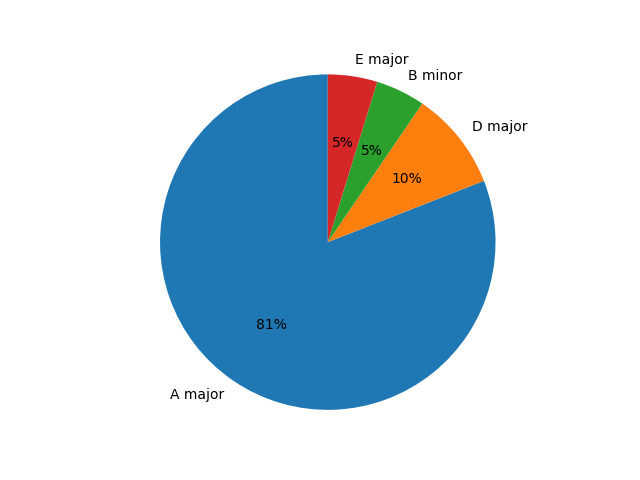
\includegraphics[width=\textwidth]{graphics/pie.png}
    \caption{Anteil der Tonarten unter Stücken des Konvoluts von Ariston Lochplatten.}
    \label{keys}
\end{figure*}

Insbesondere der letzte hörbare Akkord ist dabei für die musikwissenschaftliche Analyse von Interesse, da er üblicherweise direkte Rückschlüsse auf die Tonart des Stückes ermöglicht.
Für die Tonartbestimmung eines Stückes existieren weiterhin auch algorithmische Ansätze, wie etwa das probabilistische Modell von \textcite[]{temperley_2002}.
Die \code{musicbox} Software nutzt die Implementierung dieses Verfahrens im Python Paket music21 \parencite[]{music21} um die Tonart der Stücke auf den bearbeiteten Medien zu bestimmen.
In Abbildung \ref{keys} sind die ermittelten Tonarten für das gesamte vorhandene Konvolut von Platten des Typs Ariston zu sehen.
Die dort sichtbare Dominanz von Stücken in A-Dur im Konvolut legt den Schluss nahe, dass das Format besonders für Stücke in dieser Tonart geeignet war.
Ob dies in dem Tonvorrat den dieses Format enthält begründet liegt oder ob es sich um gesellschaftliche Gründe, wie etwa eine besonders gute Resonanz der Konsumenten auf Stücke in dieser Tonart, eventuell auch spezifisch bezogen auf Stücke die in Form solcher Toninformationsträger vertrieben wurden, handelt ist dabei eine Frage die im weiteren Lauf der musikwissenschaftliche Forschung beantwortet werden muss.

\begin{figure*}[t]
    \centering
    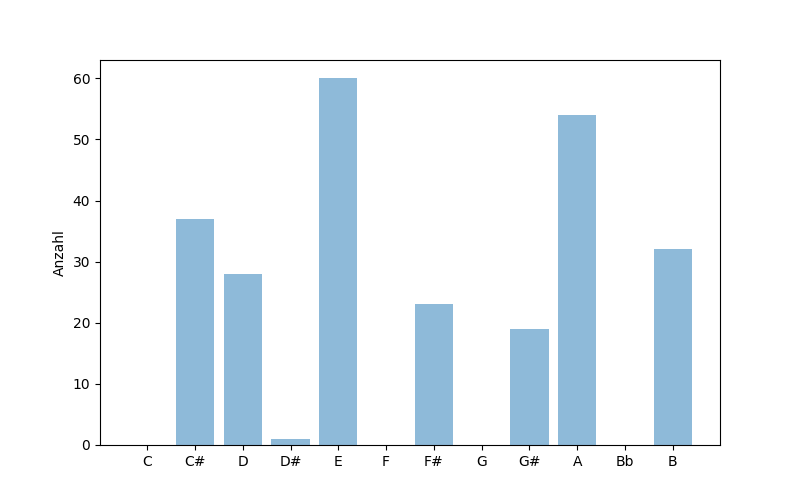
\includegraphics[width=\textwidth]{graphics/base_note_frequencies.png}
    \caption{Häufigkeit der einzelnen Grundtöne auf einer Beispielhaften Ariston Lochplatte.}
    \label{barcharts}
\end{figure*}

Neben solchen Analyseverfahren waren die beteiligten Musikwissenschaftler:innen auch an Visualisierungen zur besseren Erschließung der Medien interessiert.
Ein erster Schritt dazu ist die nach der Häufigkeit der einzelnen auf den Medien vorkommenden Tönen.
Zu diesem Zweck wurde eine Funktion implementiert, die die Notenhäufigkeit über das gesamte Medium ermittelt und als Balkendiagramm ausgibt (siehe Abbildung \ref{barcharts}).
Dabei werden durch die Software mehrere Diagramme generiert.

Zunächst wird die Häufigkeit aller Einzeltöne dargestellt, wobei die X-Achse bewusst chromatisch angeordnet ist und auch Töne einschließt die auf dem spezifischen Medium bzw. dem Medienformat insgesamt nicht vorhanden sind.
Dies dient der einfacheren optischen Erkennung von Mustern.
Ein ähnlicher Graph wird auch mit der Summe der Tonlänge pro Ton statt der Vorkommenshäufigkeit erstellt.
Um eine generalisierte Betrachtung zuzulassen werden beide Diagramme auch in einer Form erzeugt, in der die Töne auf ihre Grundtöne reduziert werden, was einen einfachere Betrachtung der Tonhäufigkeiten etwa für Rückschlüsse auf die vorkommende Tonart ermöglicht.
Zur Diagrammerstellung kommt allgemein die Python Bibliothek \code{matplotlib} \parencite[]{Hunter_2007} zum Einsatz.

\begin{figure*}[t]
    \centering
    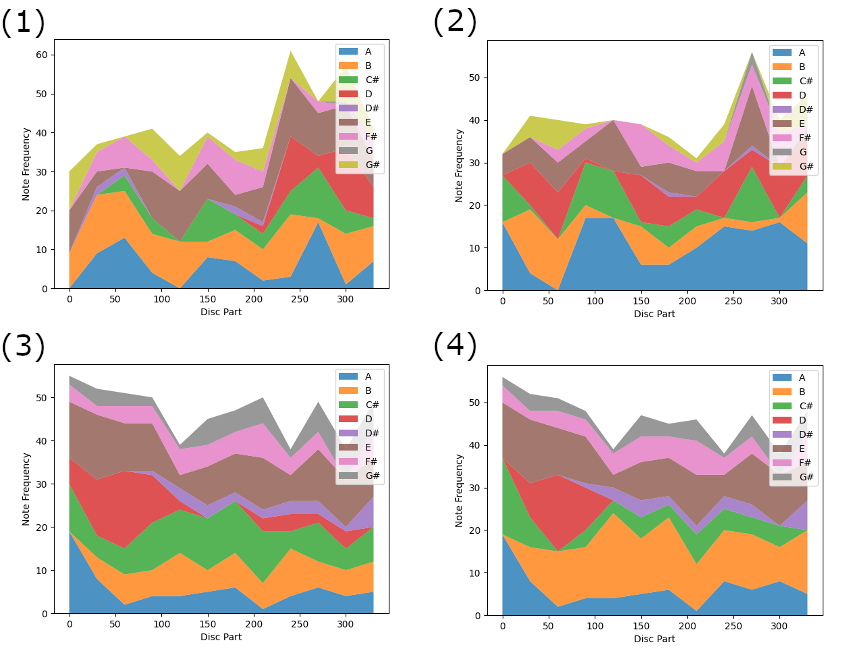
\includegraphics[width=\textwidth]{graphics/streamgraphs.png}
    \caption{Streamgraphen für 4 Lochplatten aus dem Ariston Konvolut. Platten (1) und (2) sowie Platten (3) und (4) beinhalten jeweils Fassungen des gleichen Stückes.}
    \label{streamcharts}
\end{figure*}

Die beteiligten Musikwissenschaftler:innen waren weiterhin an einer Darstellung interessiert die auch die zeitliche Komponente der Medien mit einschließt.
Hierfür wurde ein Streamgraph als Darstellungsform gewählt, der die Häufigkeit der einzelnen Grundtöne über den zeitlichen Verlauf des Mediums anzeigt.
Für die in Abbildung \ref{streamcharts} zu sehende Visualisierung mehrerer Lochplatten wurden für die vorkommenden Noten ein Binning über die zeitliche Komponente des Mediums in 12 Segmente vorgenommen.
Ferner wurden die vorkommenden Töne auf ihre Grundtöne reduziert und diese chromatisch sortiert.
So wird es ermöglicht das Musikstück auf Trends und Veränderungen in seinem zeitlichen Verlauf zu untersuchen.

Diese Streamgraph-Darstellungen haben sich auch als eine praktische Möglichkeit erwiesen eine Form von Fingerprints für einzelne Medien zu erstellen.
In Abbildung \ref{streamcharts} sind die Streamgraphen für 4 verschieden Lochplatten des Typs Ariston zu sehen.
Abgebildet sind jeweils 2 Medien von 2 unterschiedliche Musikstücken, zu denen im Bestand des Musikinstrumentenmuseums mehrere verschiedene Lochplatten vorhanden sind.
Die Lochplatten (1) und (2) enthalten beide Fassungen des Stückes \textit{An der schönen blauen Donau}, Lochplatten (3) und (4) Fassungen des \textit{Schatz-Waltzers}.
Während zwischen Lochplatten (3) und (4) leichte Unterschiede ersichtlich sind, wie etwa die Häufigkeit der Töne B und Cis, sind sich die beiden Diagramme doch strukturell sehr ähnlich, was Tonhäufigkeit und deren Entwicklung über den Verlauf der Platte betrifft.
Demgegenüber lassen Lochplatten (1) und (2) zwar noch Ähnlichkeiten erkennen, etwa der Starke anstieg an vorhandenen Tönen im letzten Abschnitt der Platte, unterscheiden sich allerdings über den gesamten Verlauf verhältnismäßig stark
Dies legt den Schluss nahe, dass Lochplatten (3) und (4) das gleiche Stück beinhalten, während es sich bei den Platten (1) und (2) potentiell um unterschiedliche Arrangements des gleichen Stückes handelt.

Neben den vorgestellten Analysemöglichkeiten erzeugt die Software während der Verarbeitung der Medien auch Reihe von Informationen die die Ergebnisse einzelner Zwischenschritte der Verarbeitung repräsentieren, etwa bildliche und textliche Daten zu gefundenen zusammenhängenden Komponenten und Noten.
Auch diese Daten lassen sich potentiell nutzen um die verarbeiteten Medien zu analysieren.
Mit tabellarischen Daten zu den erkannten Noten lassen sich beispielsweise statistische Betrachtungen der Notenlänge über verschiedene Medien realisieren.

Ebenso lassen sich durch die auf einfache Erweiterbarkeit ausgelegte Architektur der Anwendung neue Analyseschritte problemlos umsetzten und die Methoden haben nicht nur Zugriff auf die final erzeugten Midi-Daten sondern auch auf alle Daten die in Zwischenschritten erzeugt wurden.